\documentclass{article}

\usepackage{tikz}
\usepackage{xcolor}
\usepackage{pgfplots}

\usetikzlibrary{patterns}
\usetikzlibrary{shapes.geometric, arrows}
\usetikzlibrary{positioning}

\tikzstyle{decision} = [diamond, minimum width=3cm, minimum height=1cm, text centered, draw]

\begin{document}
\tikz{\draw(0,0)--(1,0)--(1,1)--(0.5,2)--(0,1)--(0,0)--(1,1)--(0,1)--(1,0);}\\
\tikz{\draw(0,0)--(5,0)--(5,5)--(2.5,10)--(0,5)--(0,0)--(5,5)--(0,5)--(5,0);}\\

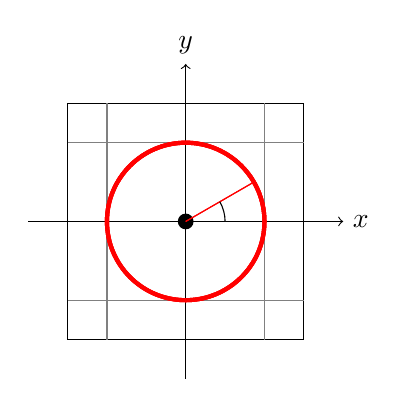
\begin{tikzpicture}
\draw(-1.5,-1.5) rectangle (1.5,1.5);
\draw[gray] (-1.5,-1.5) grid (1.5,1.5);
\draw (0,0) circle (1);
\fill (0,0) circle (0.1);
\draw[->] (-2,0) -- (2,0) node[right] {$x$};
\draw[->] (0,-2) -- (0,2) node[above] {$y$};
\draw[line width=1.5pt,red] (0,0) circle (1);
\draw[line width=1.5pt,red] (0,0) circle (1);
\draw[red] (0,0) -- ({cos(30)},{sin(30)});
\draw[line width=1.5pt,red] (0,0) circle (1);
\draw[red] (0,0) -- ({cos(30)},{sin(30)});
\draw[fill=white] ({0.5*cos(30)},{0.5*sin(30)}) arc (30:0:0.5);
\end{tikzpicture}\\

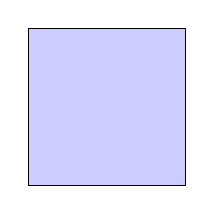
\begin{tikzpicture}
\filldraw[fill=blue!20] (0,0) rectangle (2,2);
\end{tikzpicture}\\

\tikz{\draw (0,0) -- ++(1,0) -- ++(72:1)
-- ++(144:1) -- ++(216:1) -- cycle ;}\\

\tikz{\shade[top color=red, bottom color=green,
middle color=yellow, shading angle=30]
(0,0) rectangle (1,1);}\\

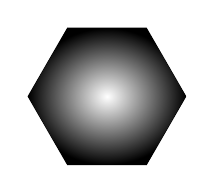
\begin{tikzpicture}
   \newdimen\R \R=1cm
   \draw (0:\R)
   \foreach \x in {60,120,...,360} { -- (\x:\R) };
   \shade[shading=radial, outer color=black,inner color=white](0:\R)
   \foreach \x in {60,120,...,360} { -- (\x:\R) };
\end{tikzpicture}\\

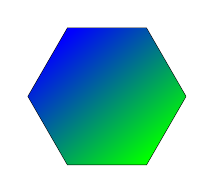
\begin{tikzpicture}
   \newdimen\R \R=1cm
   \draw (0:\R)
   \foreach \x in {60,120,...,360} { -- (\x:\R) };
   \shade[top color=blue, bottom color=green, shading angle=40](0:\R)
   \foreach \x in {60,120,...,360} { -- (\x:\R) };
\end{tikzpicture}\\

\tikz{\shade[shading=ball, ball color=gray!10, scale=2]
(0,0) circle (0.5);}\\

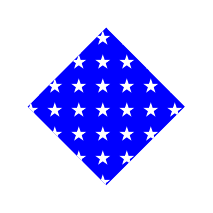
\begin{tikzpicture}
\fill[blue] (0,0) -- (45:1.41) -- (90:2) -- (135:1.41) -- cycle;
\path[pattern=fivepointed stars, pattern color=white] (0,0) -- (45:1.41) -- (90:2) -- (135:1.41) -- cycle;
\end{tikzpicture}\\

\newpage

\tikz{\draw[<-] (0,0) -- (1,0);
\draw[>-stealth] (0,-0.5) -- (1,-0.5);
\draw[|->>] (0,-1) -- (1,-1);}\\

\tikz{\path (0,0) node[circle,draw](A) {A}
(1,0) node[circle,draw](B) {B};
\node [circle,draw](C) at (3,0) {C};
\draw (A) -- (B) to[bend right] (C);}

\begin{tikzpicture}[node distance=2cm, auto]
  \node[circle,draw] (start) {START};
  \node[rectangle, draw, below=of start] (init) {i ← 1};
  \node[circle,draw, below=of init] (checkpoint) {};
  \node (dec1) [decision, below=of checkpoint] (check) {i $\leq$ 10};
  \node[rectangle, draw, below=of check] (print) {PRINT(i)};
  \node[rectangle, draw, below=of print] (inc) {INC(i)};
  \node[circle, draw, below=of inc] (stop) {STOP};

  \path[->] (start) edge (init);
  \path[->] (init) edge (checkpoint);
  \path[->] (checkpoint) edge (check);
  \path[->] (check) edge node[align=center] {igaz} (print);
  \path[->] (check) edge[bend right=60] node[align=center] {hamis} (stop);
  \path[->] (print) edge (inc);
  \path[->] (inc) edge[bend right=60] (checkpoint);
\end{tikzpicture}\\

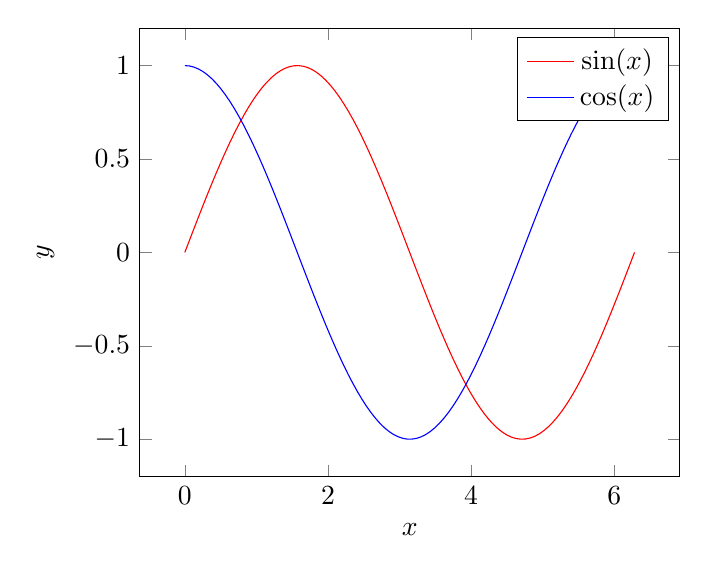
\begin{tikzpicture}
\begin{axis}[
    domain=0:2*pi,
    samples=100,
    xlabel={$x$},
    ylabel={$y$},
    legend entries={$\sin(x)$,$\cos(x)$}
]
\addplot[red] {sin(deg(x))};
\addplot[blue] {cos(deg(x))};
\legend{}
\end{axis}
\end{tikzpicture}

\end{document}